
\documentclass{svproc}
\usepackage {graphicx, amsmath, amsfonts, algorithm, algorithmic, multirow}

\begin{document}
\mainmatter
\title{Capstone Project \\ {\large Machine Learning Engineer Nanodegree}}
\author{Dennis P. F. \\ {\small December 31, 2016}}
\institute{}
%\date{December 31, 2016}
\maketitle
\pagestyle{empty}
\section{Definition}
\subsection*{Project Overview}
This project focuses on building a learning agent for LunarLander-v2 gym environment provided by OpenAI\cite{challenge}, where the agent has to navigate a space vehicle from the starting point to the landing pad on the surface of the moon without crashing.
\subsection*{Problem Statement}
The aim of the project is to build a learning agent to navigate a space vehicle from starting point in space to the landing pad without crashing. The environment is called LunarLander-v2 which is provided by OpenAI's gym python package. At each step, the agent is provided with the current state of the space vehicle $s$ which is a 8 dimensional vector of reals $\mathbb{R}^8$ and the agent is allowed to make one of four possible actions \{ \texttt{do nothing, fire left orientation engine, fire main engine, fire right orientation engine} \} in one step. On making an action $a$, the agent gets a reward $r$ and also get to know the new state of the vehicle $s'$. If the vehicle moves from the top of the screen to reach landing pad at zero speed, it gets reward in the range $[100, 140]$. The vehicle is permitted to land outside the landing pad, but is penalized for such cases. The episode finishes if the vehicle crashes(gets additional reward of -100) or comes to rest(gets additional reward of +100) which are the end states. There is an upper limit of 1000 on the number of steps in an episode. There is no restriction on the amount of fuel used. The agent is supposed to learn a policy $\pi(s)$ that decides what action it must make at a given current state $s$ by going over the past experiences defined by the tuple $<s, a, r, s'>$. The agent is considered to have solved the environment if it gets an average reward of at least 200 over 100 consecutive trials. The objective is to minimize the number of episodes required by the agent to solve the environment. Mathematically this aim can be stated as :\\\\
Minimize i such that\\\\$\frac{\displaystyle\sum_{j=i+1}^{i+100} R_j}{100} \ge 200$\\\\
and $R_j = \displaystyle\sum_{k=1}^{N_j} r_k$; $N_j \le 1000$\\\\
where $i$ and $j$ are episode indices, $R_j$ is the total reward the agent obtained in episode $j$, $k$ is the step index in a given episode and $N_j$ is the number of steps in episode $j$. $r_k$ is the reward obtained by the agent in step $k$.
\subsection*{Scoring}
The agent's score is the number of episodes needed before it completed 100 consecutive episodes over which it got an average reward of at least 200. So an agent that learns faster with minimum number of episodes and solves is considered better than an agent that solves the problem only after learning for larger number of episodes.
\section{Analysis}
\subsection*{Data Exploration}
The state space is $\mathbb{R}^8$. The first two dimensions indicate the coordinates of the vehicle. Third and fourth dimensions indicate x and y components of the velocity of the vehicle. Fifth component specifies angle between lander pad and the vehicle base. Sixth component gives the angular velocity with respect to lander pad. Seventh and eighth dimensions indicate whether the legs of the vehicle has made ground contact or not. There are four discrete actions that the agent can make in one step : \{ \texttt{do nothing, fire left orientation engine, fire main engine, fire right orientation engine} \}.The vehicle always starts at top middle of the screen in every episode and the lander pad is always at coordinates (0,0). The episode ends when the vehicle reaches any of its end states : 1) lands on the landing pad with zero speed 2) vehicle crashes. It is assumed that state observation made by the agent is accurate however no assumption is made as to whether the state transition is deterministic with respect to any action made by the agent.
\subsection*{Exploratory Visualization}
Following bar-charts show the mean and standard deviation of the 8 state space components in an experiment where a random action was chosen in each step per episode for 500 such episodes.\\
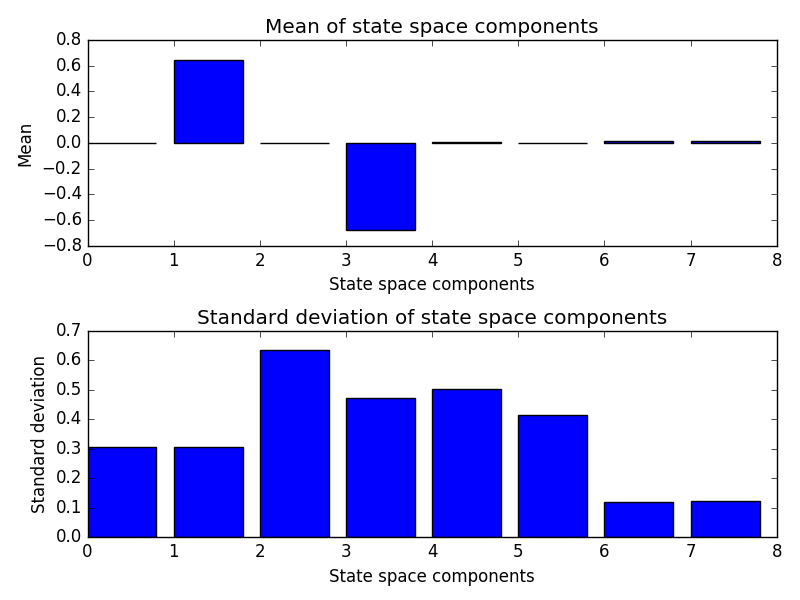
\includegraphics[width=11cm]{img/state-space}\\
The bar-charts indicate that the y coordinate(index 1) of the vehicle and y component of velocity(index 3) have their mean away from 0 while all other components have mean close to 0. Second plot indicate relatively higher standard deviation in x component of the vehicle's velocity and lower value for last two components of state space.
\subsection*{Algorithms and Techniques}
The problem at hand is a good case for using Reinforcement Learning approach. Q-learning is one of the algorithms in reinforcement learning but is limited to problems with discrete state and action spaces. In this case the state space is 8 dimensional and continuous. Discretization of state space is inefficient and the memory requirement grows exponentially with number of discrete units chosen per state dimension. This project make use of a relatively recent technique called Deep Q Network(DQN)\cite{DQN} which is thoroughly explained in the blog by Jaromír Janisch\cite{Jaromir}. DQN uses a neural network that learns to approximate the function 
$Q^*(s, a)$ which is the total reward the agent will achieve starting at state $s$, then takes action $a$ then following the policy\\\\$\pi(s) = argmax_a Q^*(s, a)$\\\\
The true Q function can be written in terms of rewards as\\\\$Q^*(s, a) = \sum_{i=0}^{\infty} \gamma^i r_i$\\\\ where $\gamma$ is the discount factor with the constraint $0 < \gamma < 1$. This ensures that the sum in the formula for $Q^*(s, a)$ is finite valued. $\gamma$ determines how much Q of current state depends on future. In DQN the neural network accepts the state as input and produces the estimated Q values for each action. Such a network is trained by using $<s, a, r, s'>$ tuples the agent experienced in past and making use of Bellman recursive formulation of $Q^*(s, a)$ given by :\\\\
$Q^*(s, a) = r + \gamma \max_a Q^*(s', a)$\\\\
From an experience tuple $<s, a, r, s'>$ the neural network approximation of $Q^*(s,a)$ can be improved/trained as follows
\vspace{-0.09cm}
\begin{enumerate}
	\item Compute the Q values for state $s$ for all actions $a'$ by using a forward pass of the neural net.\\$q_{a'} = Q(s, a') \quad \forall a'$\\
	\item Compute the Q values for state $s'$ for all actions $a'$ by using a forward pass of the neural net.\\$p_{a'} = Q(s', a') \quad \forall a'$\\
	\item Compute the target Q values for state $s$ to construct a training example for the Q network as :\\
	Set $t_{a'} = q_{a'} \forall a' \neq a$\\Set $ t_{a} = \begin{cases} r + \gamma \max_{a'}p_{a'} & \text{s is not the end state}\\ r & \text{s is the end state}        \end{cases}$\\ The training example is now $\{s, (t_1, t_2, ..., t_k)\}$ where $k$ is the total number of actions.
\end{enumerate}
The Q approximation neural network is trained using these generated training examples via back-propagation using Adam\cite{adam} optimizer. The agent stores the experience tuples $<s, a, r, s'>$ in a memory buffer which can store $100000$ such tuples. The neural network is trained in every step by randomly sampling 32 tuples from this buffer. This technique is referred to as \textit{experience replay} in the original DQN paper. For making actions in each step the agent follows a $\epsilon$-greedy method in which the agent makes random action with probability $\epsilon$ and uses the Q network's outputs to decide best actions (greedy) with probability $1-\epsilon$. Initially $\epsilon$ is set to $1.0$ (full exploration) and then decayed exponentially by a factor of $0.995$.
\subsection*{Benchmark}
An agent which chooses random action every step is chosen as the baseline algorithm. This algorithm does not learn from past experiences and is expected not to solve the environment with a very high probability. The basic DQN algorithm is compared against its different variations/improvements.
The baseline algorithm RandomAgent can be run as:\\
\texttt{\\\$ cd src}
\texttt{\\\$ python run\_random\_agent.py}\\\\
Below plots shows the performance of random agent a) in terms of the reward earned per episode for 500 episodes and b) number of steps in each episode.\\
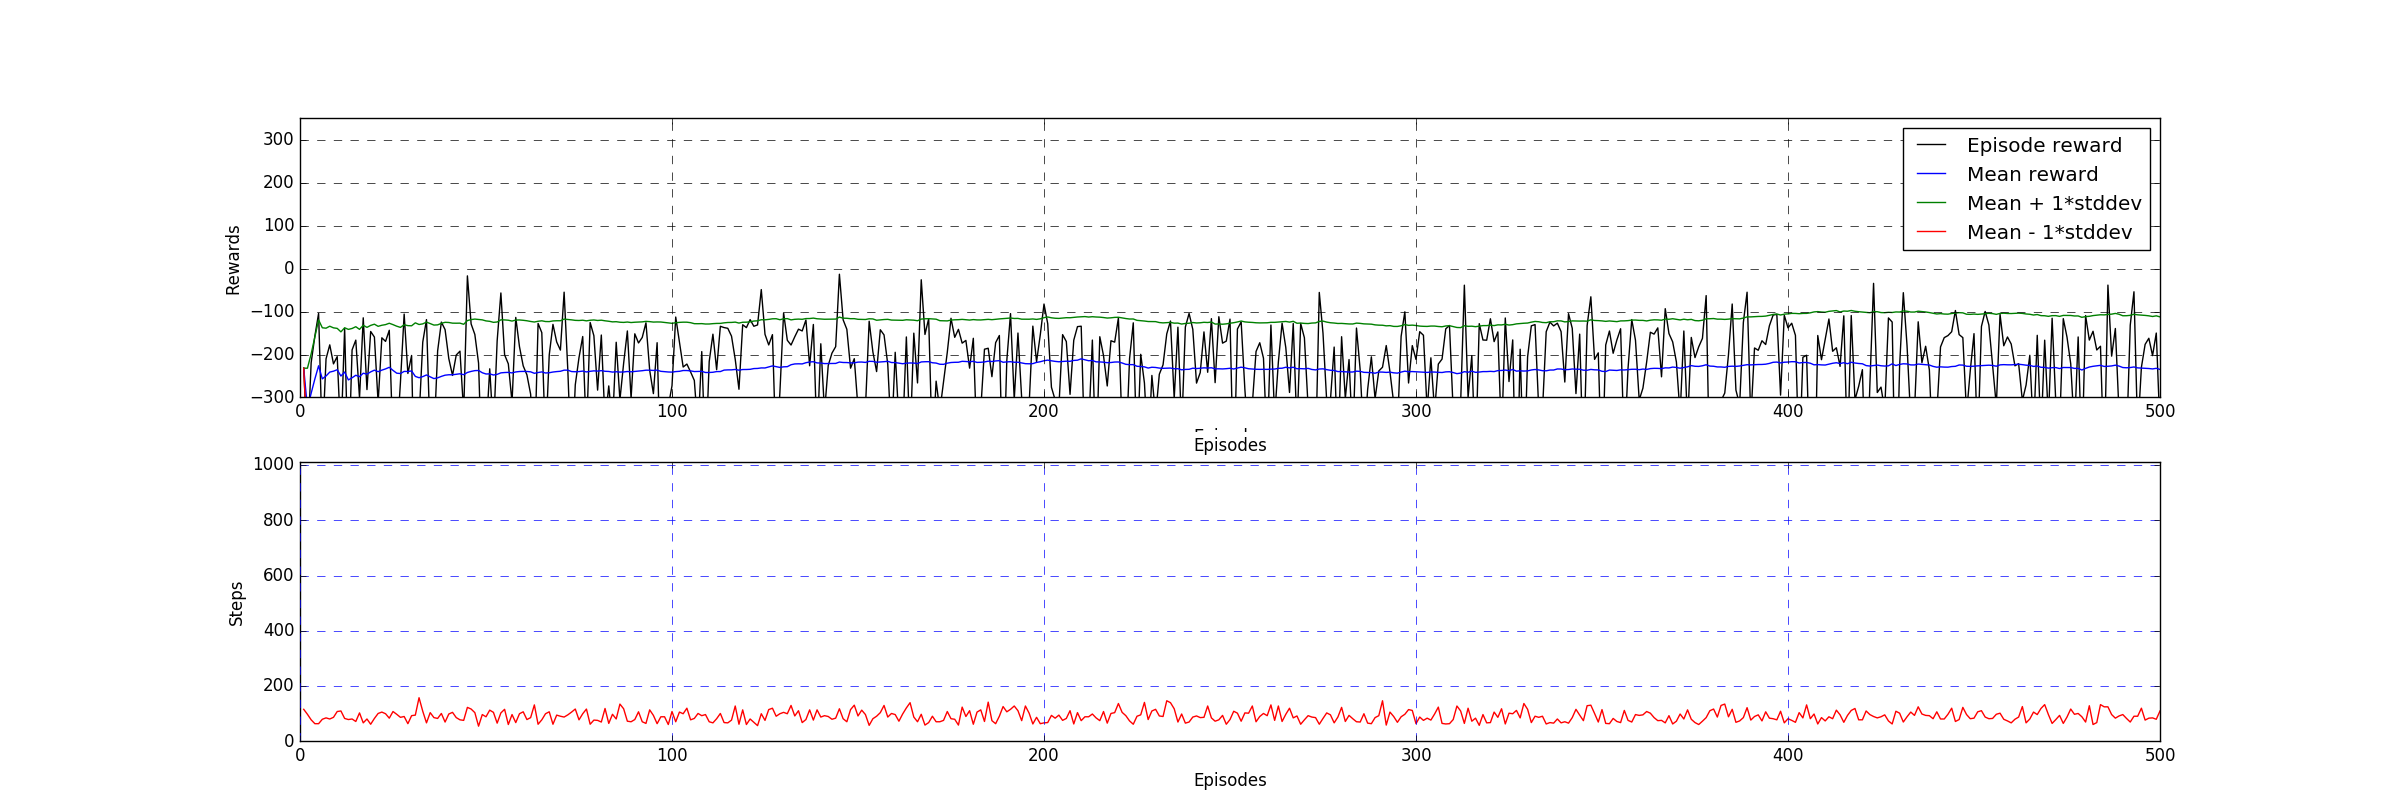
\includegraphics[width=14cm,trim={5cm 0 0 0},clip]{img/randomagent}\\
As expected the agent was not able to achieve rewards greater than $0$ in any of the episodes with mean reward under $-200.0$ indicating that the vehicle crashed in most cases. Another fact is that episode length in general is well below 200 steps.
\section{Methodology}
\subsection*{Data Processing}
\subsection*{Implementation}
\section{Results}
\section{Conclusion}
\begin{thebibliography}{}
\bibitem{challenge}
LunarLander-v2 gym environment provided by OpenAI - \texttt{https://gym.openai.com/envs/LunarLander-v2}
\bibitem{DQN}
Mnih, Volodymyr, et al. "Human-level control through deep reinforcement learning." Nature 518.7540 (2015): 529-533.
\bibitem{Jaromir}
Let’s make a DQN - blog series by Jaromír Janisch - \texttt{https://jaromiru.com/2016/09/27/lets-make-a-dqn-theory/}
\bibitem{adam}
Kingma, Diederik, and Jimmy Ba. "Adam: A method for stochastic optimization." arXiv preprint arXiv:1412.6980 (2014).
\end{thebibliography}

\end{document}
